\chapter{Comparative Evidence Across Model Classes}\label{ch:results}
The models can now be compared through a common set of questions: what happens to execution revenue, inventory exposure, terminal liquidation and the control equation? Comparisons are paired within a declared experiment. Absolute PnL across rows is not a common score: terminal costs, control bounds, initialization and simulation designs differ. The diffusion benchmark uses terminal marked wealth, while the liquidation experiments deduct a declared close-out cost once.

\section{Markovian diffusion benchmarks}



\subsection{Single-Asset Monte Carlo Diagnostics}

The single-asset experiment uses $N=5{,}000$ Monte Carlo paths, $T=1$, $1{,}000$ time steps, $S_0=100$, $\gamma=0.1$, $k=1.5$, $A=140$, and the optimal liquidity half-spread
\[
\delta^*=
\frac{1}{\gamma}\log\!\left(1+\frac{\gamma}{k}\right)
=
0.6454.
\]
The ABM volatility is $\sigma_{ABM}=1.5$. The GBM volatility is calibrated as $\sigma_{GBM}=0.015$, so that $\sigma_{GBM}S_0=\sigma_{ABM}$ and both models have the same initial dollar volatility.

\begin{table}[H]
\centering
\small
\caption{Single-asset Monte Carlo diagnostics with $5{,}000$ simulated paths and inventory-based improvement relative to naive quoting. Negative values in inventory and volatility metrics indicate risk reduction.}
\begin{tabular*}{\textwidth}{@{\extracolsep{\fill}}l!{\vrule width 0.5pt}rrr!{\vrule width 0.5pt}rrr@{}}
\toprule
Metric & ABM Naive & ABM AS & Difference & GBM Naive & GBM AS & Difference \\
\midrule
Mean terminal PnL        & 67.145 & 63.930 & -3.215 & 67.109 & 63.894 & -3.215 \\
Std terminal PnL         & 12.178 &  6.680 & -5.498 & 12.316 &  6.718 & -5.598 \\
Sharpe-like ratio        &  5.514 &  9.570 &  4.056 &  5.449 &  9.511 &  4.062 \\
Mean $|$terminal inv$|$  &  7.817 &  3.116 & -4.701 &  7.897 &  3.095 & -4.802 \\
Mean Std$(q_t)$          &  3.708 &  1.799 & -1.909 &  3.727 &  1.795 & -1.932 \\
Mean turnover            &103.845 &107.414 &  3.569 &103.618 &107.298 &  3.680 \\
\bottomrule
\end{tabular*}
\end{table}

The central result is not that the inventory-based dealer always maximizes raw terminal PnL path by path. In the ABM and GBM Monte Carlo tables, the naive dealer has a slightly higher average terminal PnL, roughly $3.2$ units more in both models. This is expected in a simplified simulator without adverse selection, market impact, fees, or hard inventory limits: a symmetric dealer can sometimes earn more gross spread by accepting larger inventory risk.

The relevant advantage of the Avellaneda--Stoikov rule is risk adjustment. Under ABM, the standard deviation of terminal PnL falls from $12.178$ to $6.680$, while the Sharpe-like ratio rises from $5.514$ to $9.570$. The mean absolute terminal inventory falls from $7.817$ to $3.116$, and the average intraday inventory standard deviation is almost halved. The GBM case produces the same qualitative pattern: lower PnL dispersion, lower terminal inventory, lower intraday inventory variability, and a much higher Sharpe-like ratio. The slight increase in turnover is consistent with the mechanism of the strategy: the AS dealer actively skews quotes to encourage inventory-reducing trades.

\begin{figure}[H]
\centering
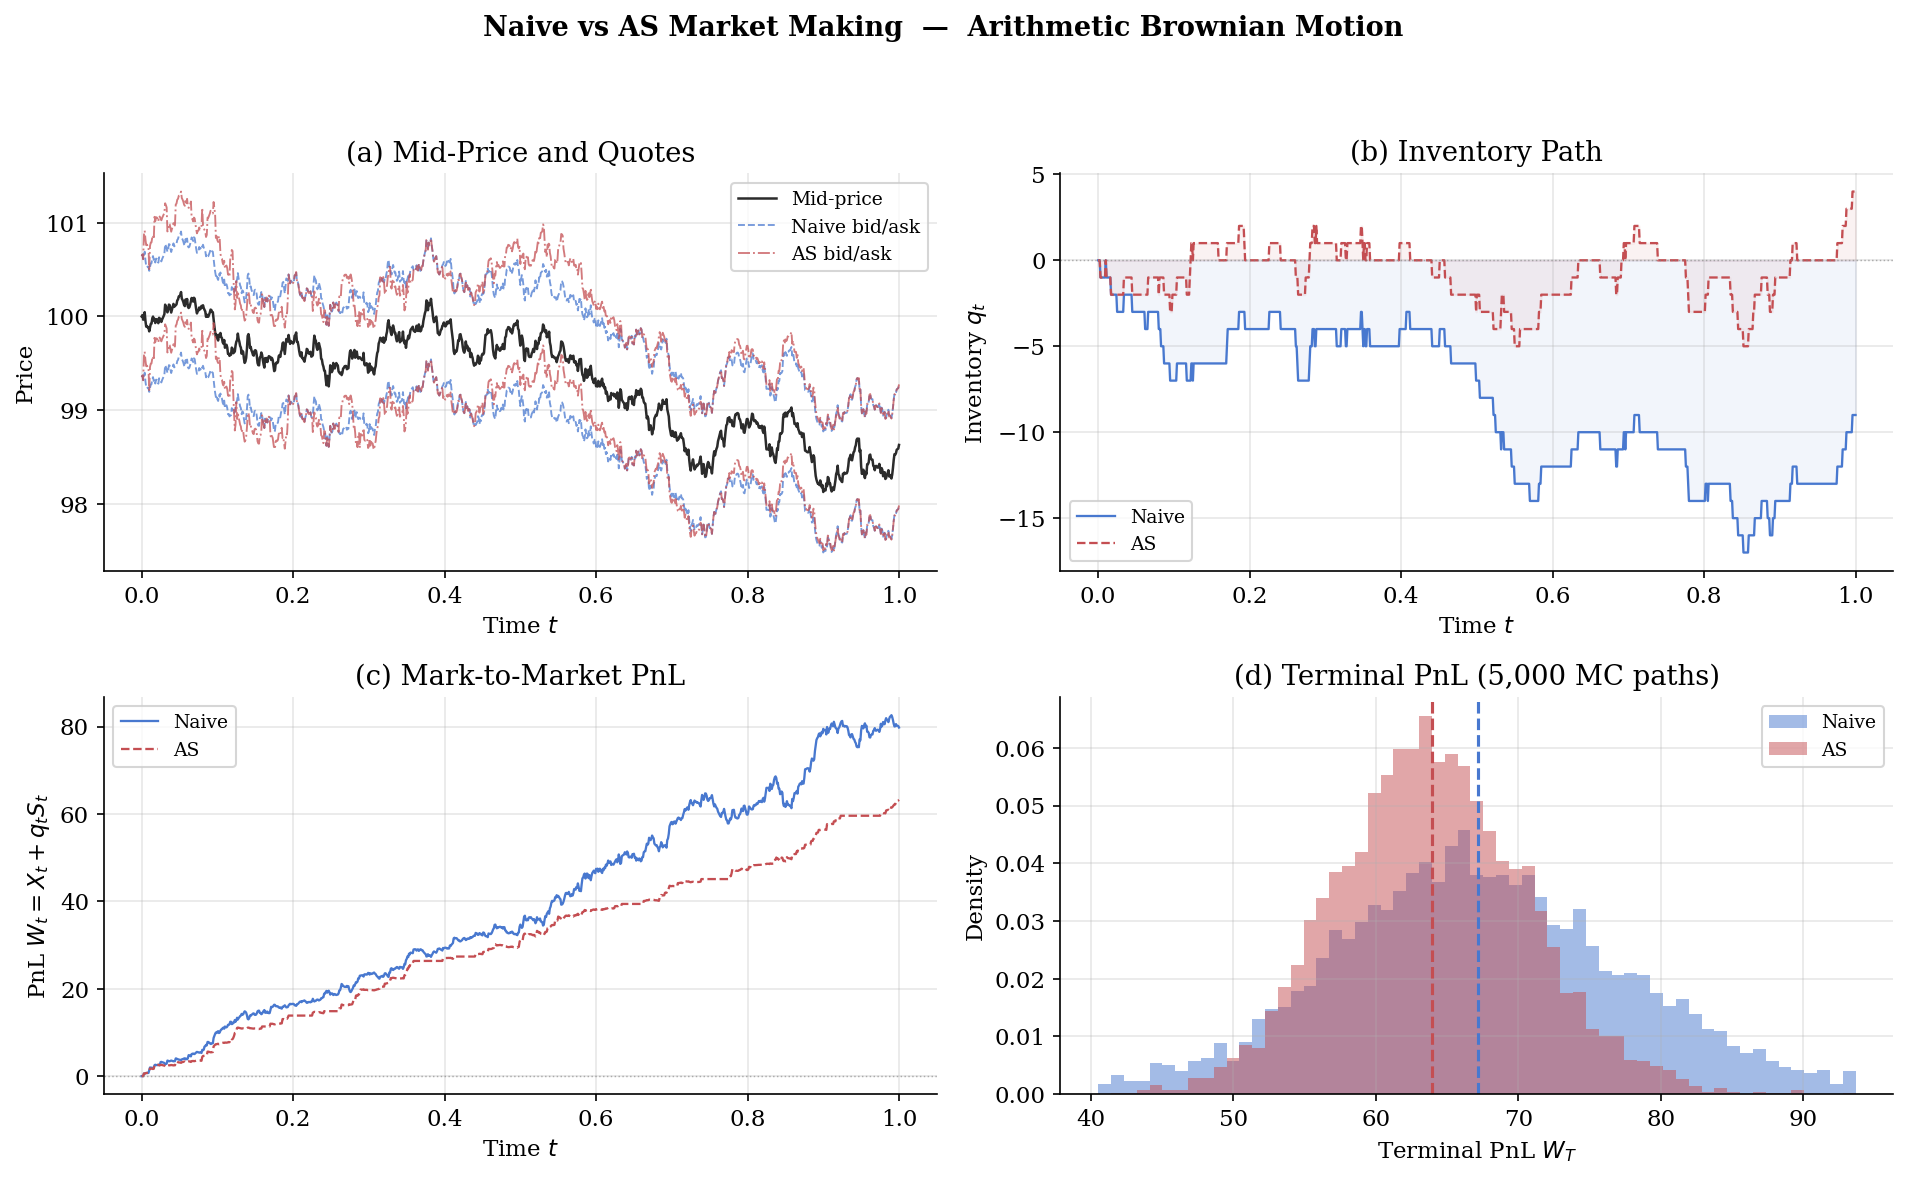
\includegraphics[width=0.85\textwidth]{img/hft1-py1.png}
\caption{Single-asset ABM comparison: naive versus Avellaneda--Stoikov quoting.}
\label{hft1-fig:bm_results}
\end{figure}

Figure~\ref{hft1-fig:bm_results} illustrates the ABM case. Panel (a) shows that both strategies quote around the same mid-price, but the AS quotes are not fixed symmetrically around $S_t$: they move with inventory through the reservation-price adjustment. When the dealer accumulates a long inventory, the quote center is pushed downward to make selling more likely and further buying less attractive; when the dealer is short, the opposite adjustment occurs. Panel (b) makes this mechanism visible. The naive inventory drifts much further from zero because the policy has no endogenous force pulling $q_t$ back toward neutrality, while the AS inventory is actively stabilized by the quote skew. Panel (c) should be read as a single realized path, not as the main performance criterion. In this particular path, the naive strategy ends higher because the realized price movement happens to reward the inventory exposure it has accumulated. Panel (d) is therefore the more relevant diagnostic: over $5{,}000$ paths, the naive terminal PnL distribution is wider, whereas the AS distribution is more concentrated. The message is that the AS rule does not simply try to maximize one lucky path; it reduces the dispersion generated by unmanaged inventory exposure.

\begin{figure}[H]
\centering
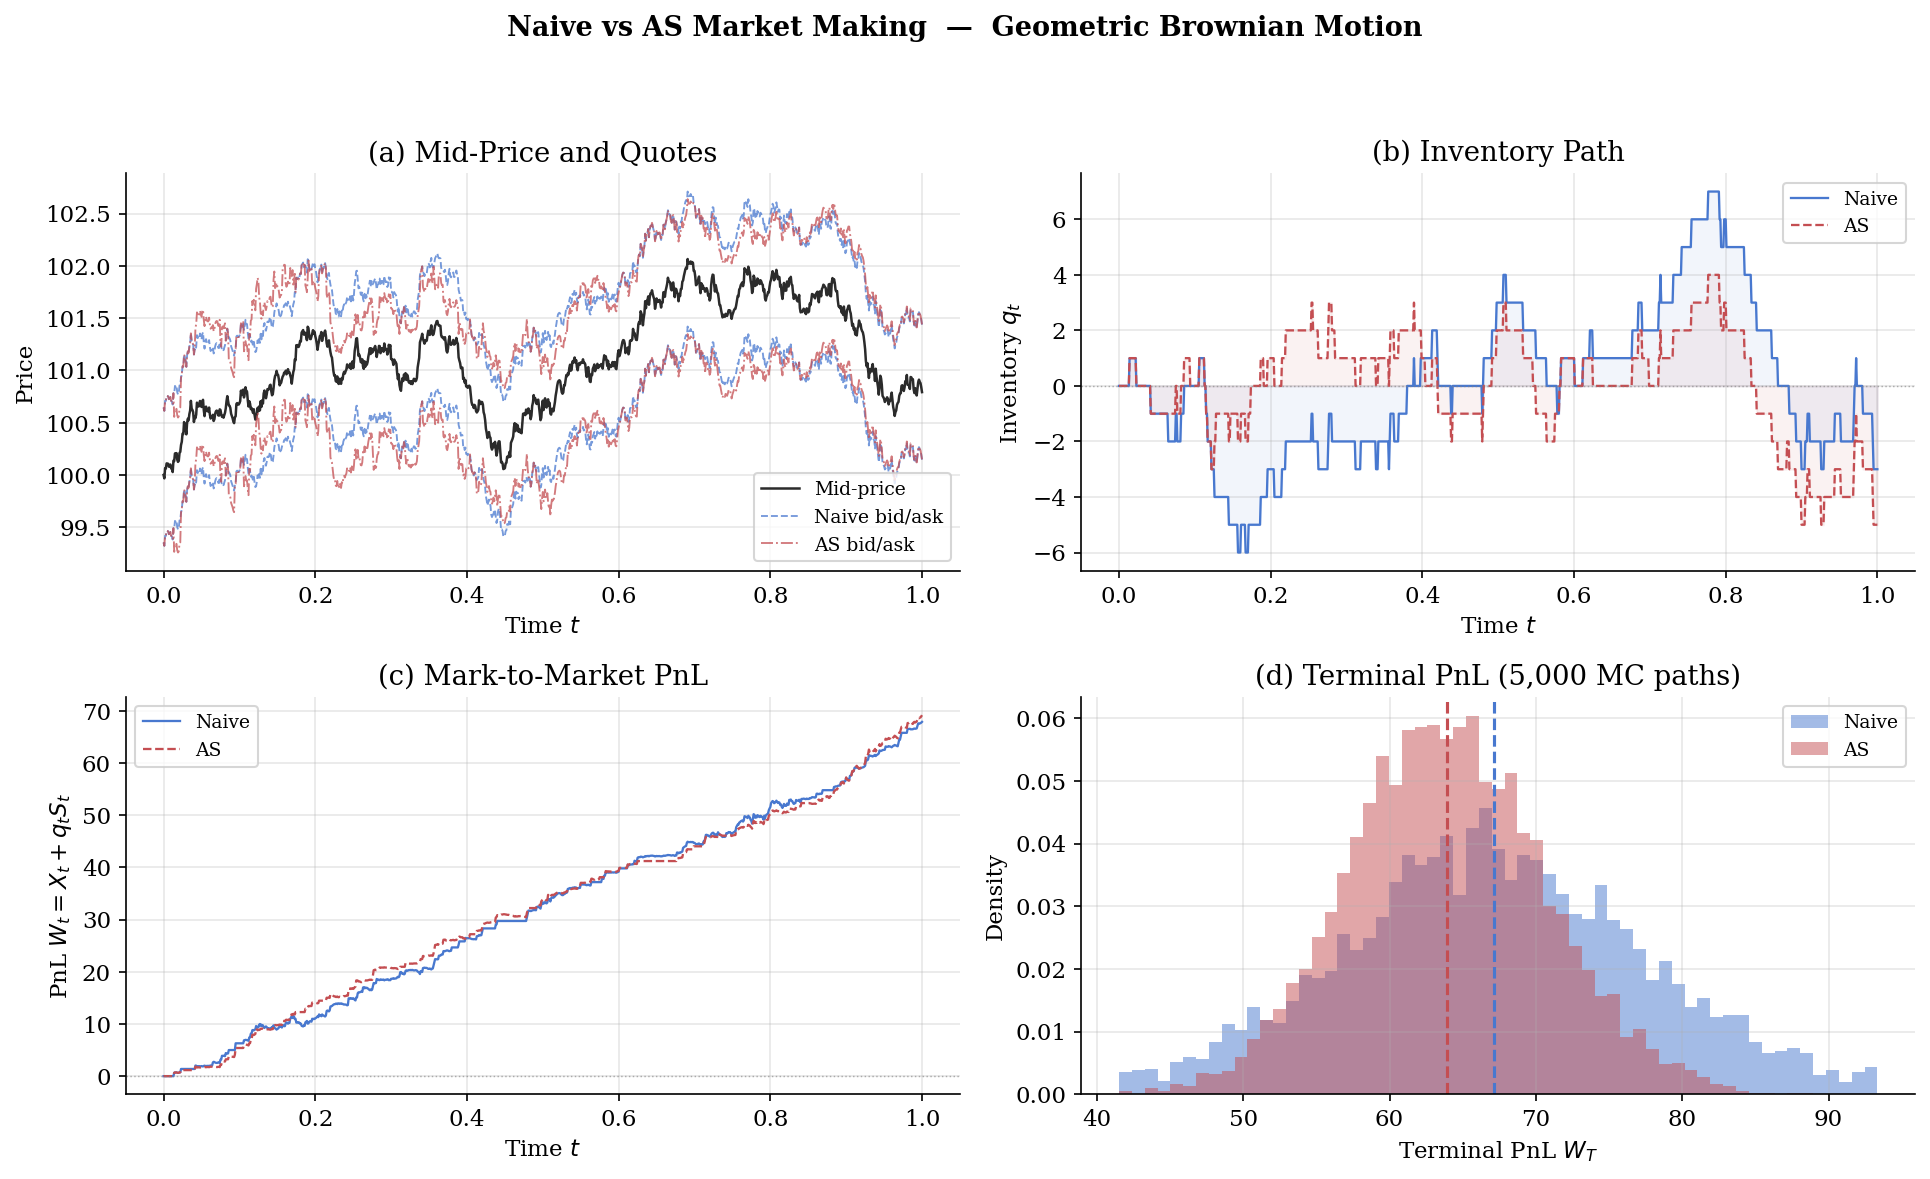
\includegraphics[width=0.85\textwidth]{img/hft1-py2.png}
\caption{Single-asset GBM comparison: naive versus Avellaneda--Stoikov quoting.}
\label{hft1-fig:gbm_results}
\end{figure}

Figure~\ref{hft1-fig:gbm_results} reports the GBM case. Since $\sigma_{GBM}S_0$ is calibrated to match the ABM dollar volatility, the aggregate Monte Carlo diagnostics are close to the ABM case. The difference is conceptual rather than cosmetic. Under GBM, the volatility parameter describes return risk, while the risk of holding one physical unit of inventory depends on the current price level. For this reason, the simulation uses the local monetary variance approximation $(\sigma_{GBM}S_t)^2$ inside the reservation price. When $S_t$ increases, one unit of inventory becomes riskier in dollar terms, and the AS quote skew reacts more strongly. This is why the GBM version is useful even if the numerical table is similar to ABM: it shows that inventory control should be expressed in monetary-risk units, not directly in return-volatility units.

\subsection{Covariance-Aware Multi-Asset Diagnostics}

The multivariate experiment uses three correlated arithmetic Brownian assets. Asset C is deliberately specified as inversely correlated with the first two assets, so that the covariance pressure $\Sigma q_t$ can differ sharply from the raw inventory vector $q_t$. This makes the key multi-asset mechanism visible: a position that looks large in physical units may be less dangerous if it hedges the rest of the book, while a small position may still be risky if it loads on the same covariance direction as the current portfolio.

\begin{figure}[H]
\centering
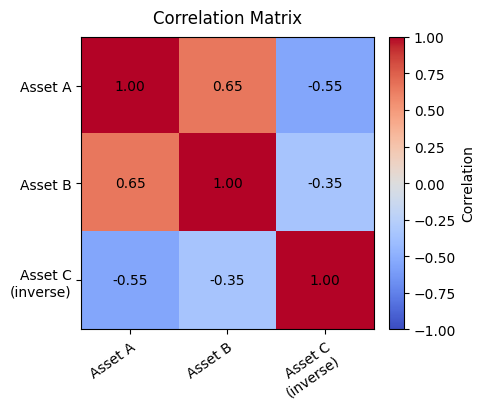
\includegraphics[width=0.58\textwidth]{img/hft1-Corr.png}
\caption{Correlation matrix used in the three-asset diagnostic. The matrix has unit diagonal entries, with $\rho_{AB}=0.65$, $\rho_{AC}=-0.55$, and $\rho_{BC}=-0.35$. Positive values indicate co-movement between assets, while negative values capture the inverse exposure of Asset C.}
\label{hft1-fig:correlation-matrix-three-asset}
\end{figure}

The corresponding covariance matrix $\Sigma$ combines these correlation coefficients with the individual asset volatilities. It is the matrix used by the covariance-aware policy to transform the raw inventory vector $q_t$ into the risk-pressure vector $\Sigma q_t$.

\begin{table}[H]
\centering
\small
\caption{Covariance matrix $\Sigma$ used in the three-asset diagnostic.}
\begin{tabular}{@{}lrrr@{}}
\toprule
 & Asset A & Asset B & Asset C (inverse) \\
\midrule
Asset A           &  2.2500 &  1.0725 & -0.7425 \\
Asset B           &  1.0725 &  1.2100 & -0.3465 \\
Asset C (inverse) & -0.7425 & -0.3465 &  0.8100 \\
\bottomrule
\end{tabular}
\end{table}

For $N=3{,}000$ Monte Carlo paths, the covariance-aware inventory policy again sacrifices a small amount of average PnL but materially improves the risk profile of the terminal book.

\begin{table}[H]
\centering
\small
\caption{Multivariate Monte Carlo diagnostics with $3{,}000$ simulated paths.}
\begin{tabularx}{\textwidth}{@{}Xrrr@{}}
\toprule
Metric & Naive & Inventory-based & Difference \\
\midrule
Mean terminal PnL                         & 158.709 & 154.556 & -4.153 \\
Std terminal PnL                          &  16.439 &  10.547 & -5.892 \\
Sharpe-like ratio                         &   9.654 &  14.654 &  5.000 \\
Mean $|$terminal inv$|$                   &  21.949 &  11.203 & -10.745 \\
Mean Std$(q_t)$                           &   6.593 &   3.397 & -3.195 \\
Mean turnover                             & 266.641 & 257.767 & -8.874 \\
Mean terminal risk $\|q_T\|_\Sigma$       &  17.051 &   7.419 & -9.632 \\
Median terminal risk $\|q_T\|_\Sigma$     &  15.313 &   6.996 & -8.318 \\
Mean average path risk                    &  11.397 &   3.925 & -7.472 \\
Mean max path risk                        &  22.638 &  10.065 & -12.573 \\
\bottomrule
\end{tabularx}
\end{table}

The multivariate results are stronger than the single-asset results because the naive policy is not merely ignoring inventory size; it is ignoring the entire covariance structure. The mean terminal risk norm $\|q_T\|_\Sigma=\sqrt{q_T^\top\Sigma q_T}$ falls from $17.051$ to $7.419$, while the mean maximum path risk falls from $22.638$ to $10.065$. The average gross terminal inventory also falls by more than ten units. These diagnostics show that covariance-aware control does not simply reduce each position mechanically; it reduces the risk of the portfolio after correlations are taken into account.

\begin{figure}[H]
\centering
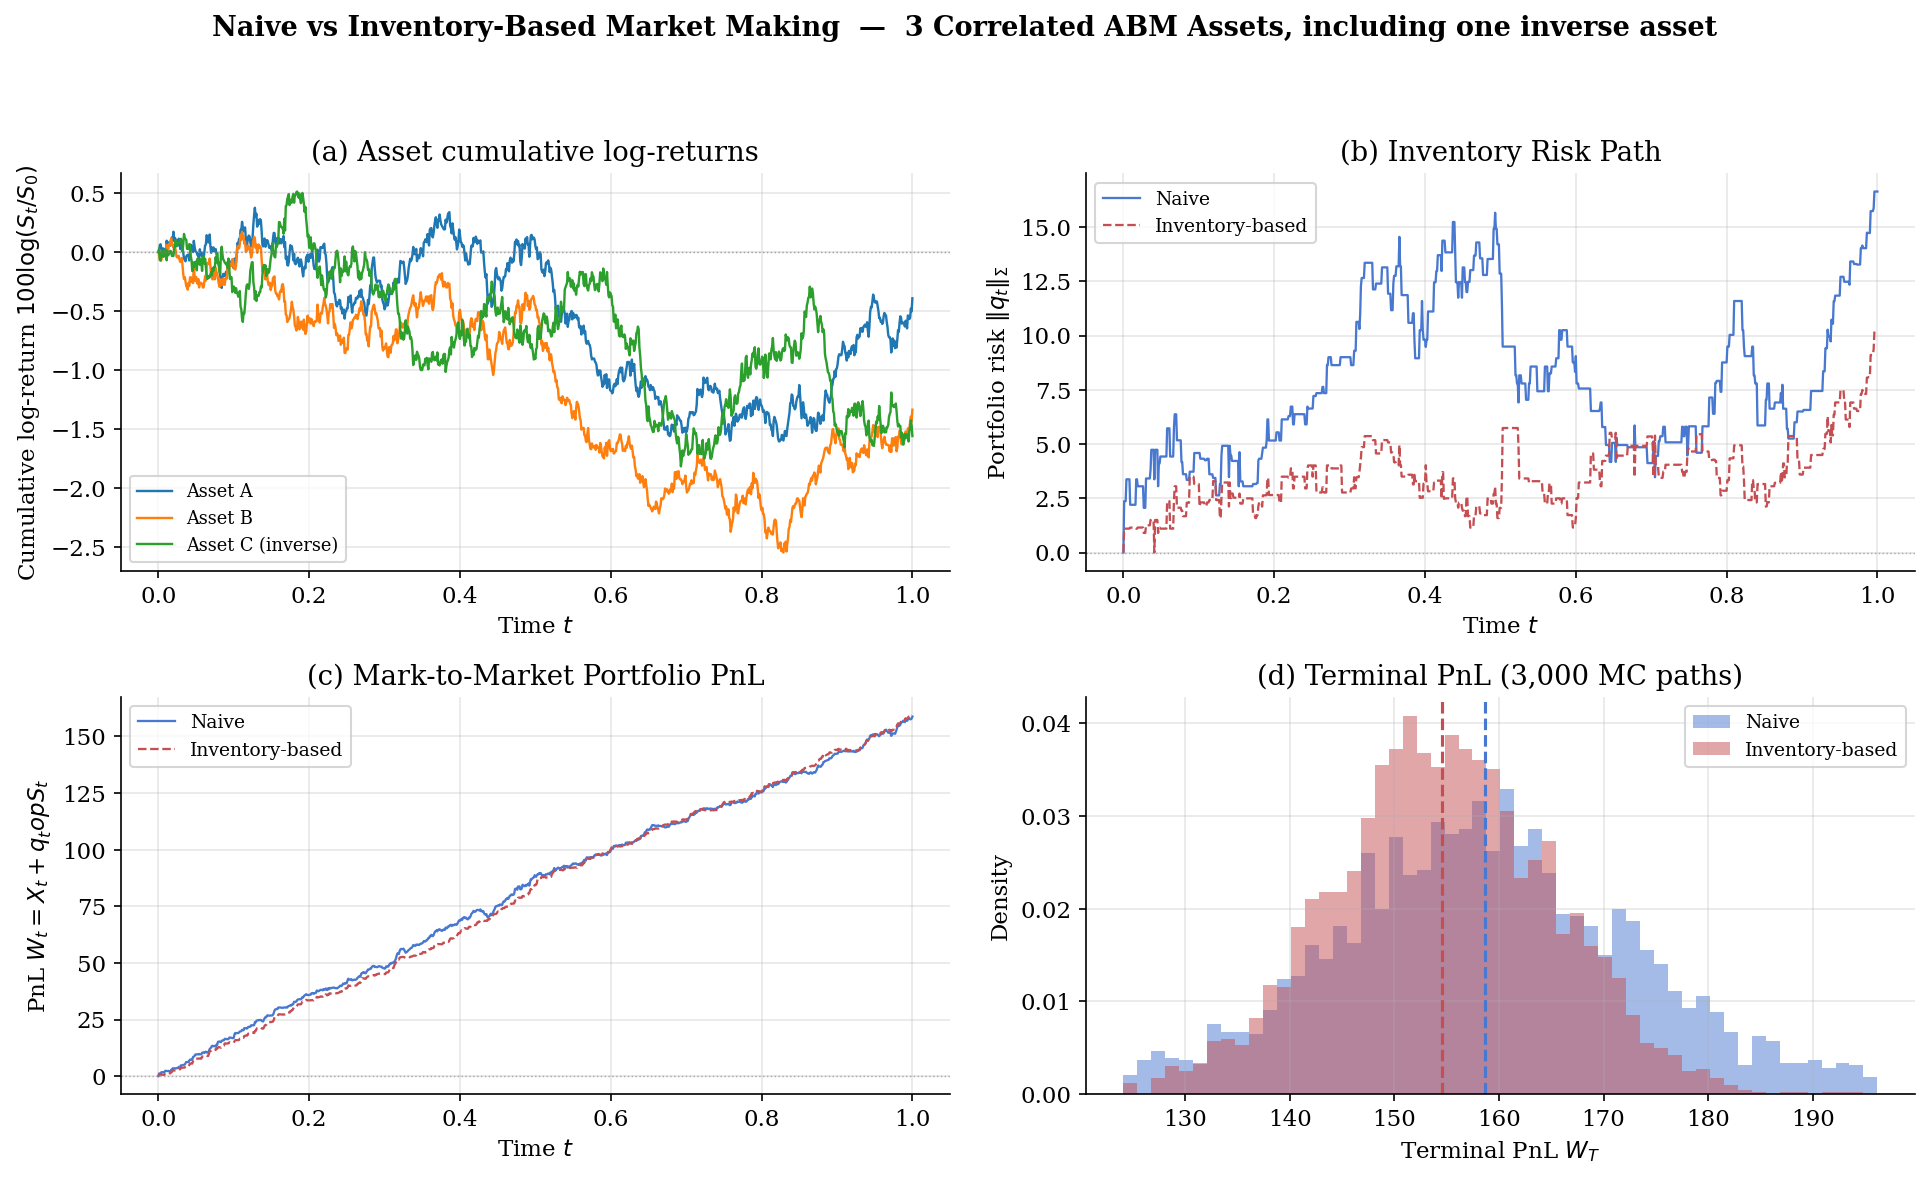
\includegraphics[width=0.96\textwidth]{img/hft1-py3.png}
\caption{Three-asset covariance-aware market-making diagnostic.}
\label{hft1-fig:multi_results}
\end{figure}

Figure~\ref{hft1-fig:multi_results} summarizes the three-asset diagnostic. Panel (a) reports cumulative log-returns, which makes the three price paths comparable even though the assets start from different price levels. The third asset is intentionally inversely correlated with the first two, so the relevant inventory signal is no longer the raw vector $q_t$ alone but the covariance-adjusted pressure $\Sigma q_t$. Panel (b) shows the portfolio risk norm $\|q_t\|_\Sigma$, which is the natural multivariate analogue of single-asset inventory risk. The naive strategy accumulates a much larger covariance-adjusted exposure because it treats each asset independently, while the inventory-based strategy keeps the risk path lower by reacting to the whole book. Panel (c) shows that both policies generate positive spread-capture PnL on the reference path, but the inventory-aware policy does so with a substantially lower portfolio-risk footprint. Panel (d) confirms the Monte Carlo result: the inventory-based terminal PnL distribution is more concentrated, while the naive policy leaves wider tails because it accepts larger covariance-adjusted inventory exposure. This is the key difference from the scalar case: the multi-asset dealer must control the risk of the book, not only the size of each single position.

Overall, the numerical evidence is consistent across all three experiments. The naive policy can look attractive if one only checks average PnL in a frictionless benchmark, but this comes from carrying more inventory risk. The Avellaneda--Stoikov policy is better understood as a risk-adjusted market-making rule: it reduces terminal inventory, lowers PnL volatility, and becomes especially valuable once the dealer manages a correlated book rather than a single isolated asset.

These covariance-aware diffusion results establish the inventory-risk mechanism before volatility memory and terminal liquidation are introduced in the next experiment.

The common finding in ABM, local-variance GBM and the correlated diffusion is reduced exposure and dispersion, with a lower mean PnL in the displayed samples. This does not establish a benefit from memory: none of these environments contains a rough volatility state. We therefore turn to a different experiment with a finite memory approximation and priced terminal liquidation.
\section{Finite-lift configurations with historical scalar controls}
The following 2000-session results use the historical clipped scalar solver and full finite-lift forward paths. They are retained as evidence for that implementation, not as a converged optimal-policy benchmark. Their $H$ labels refer to the weight prescription explained in Chapter~\ref{ch:control}.
\subsection{Diagnostics, figures, and representative close-out paths}

The numerical pipeline produces the diagnostics and the two figures included below. Figure~\ref{hft2-fig:hjb_surfaces} reports the initial HJB surfaces for all three Hurst regimes. These panels are easy to misread on a first pass, so it is useful to separate the interpretation carefully.

\begin{algorithm}[H]
\caption{Reading the HJB surface figure}
\DontPrintSemicolon
\For{each \(H\in\{0.2,0.5,0.8\}\)}{
  calibrate the lifted rough environment and compress it to the HJB state \(y\)\;
  solve the reduced HJB backward on the \((q,y)\) grid with liquidation terminal condition\;
  export \(\Theta(0,q,y)\), \(\delta^{b,*}(0,q,y)\), and \(\delta^{a,*}(0,q,y)\)\;
}
read rows by regime and columns by continuation value, bid offset, and ask offset\;
\end{algorithm}

\begin{figure}[H]
\centering
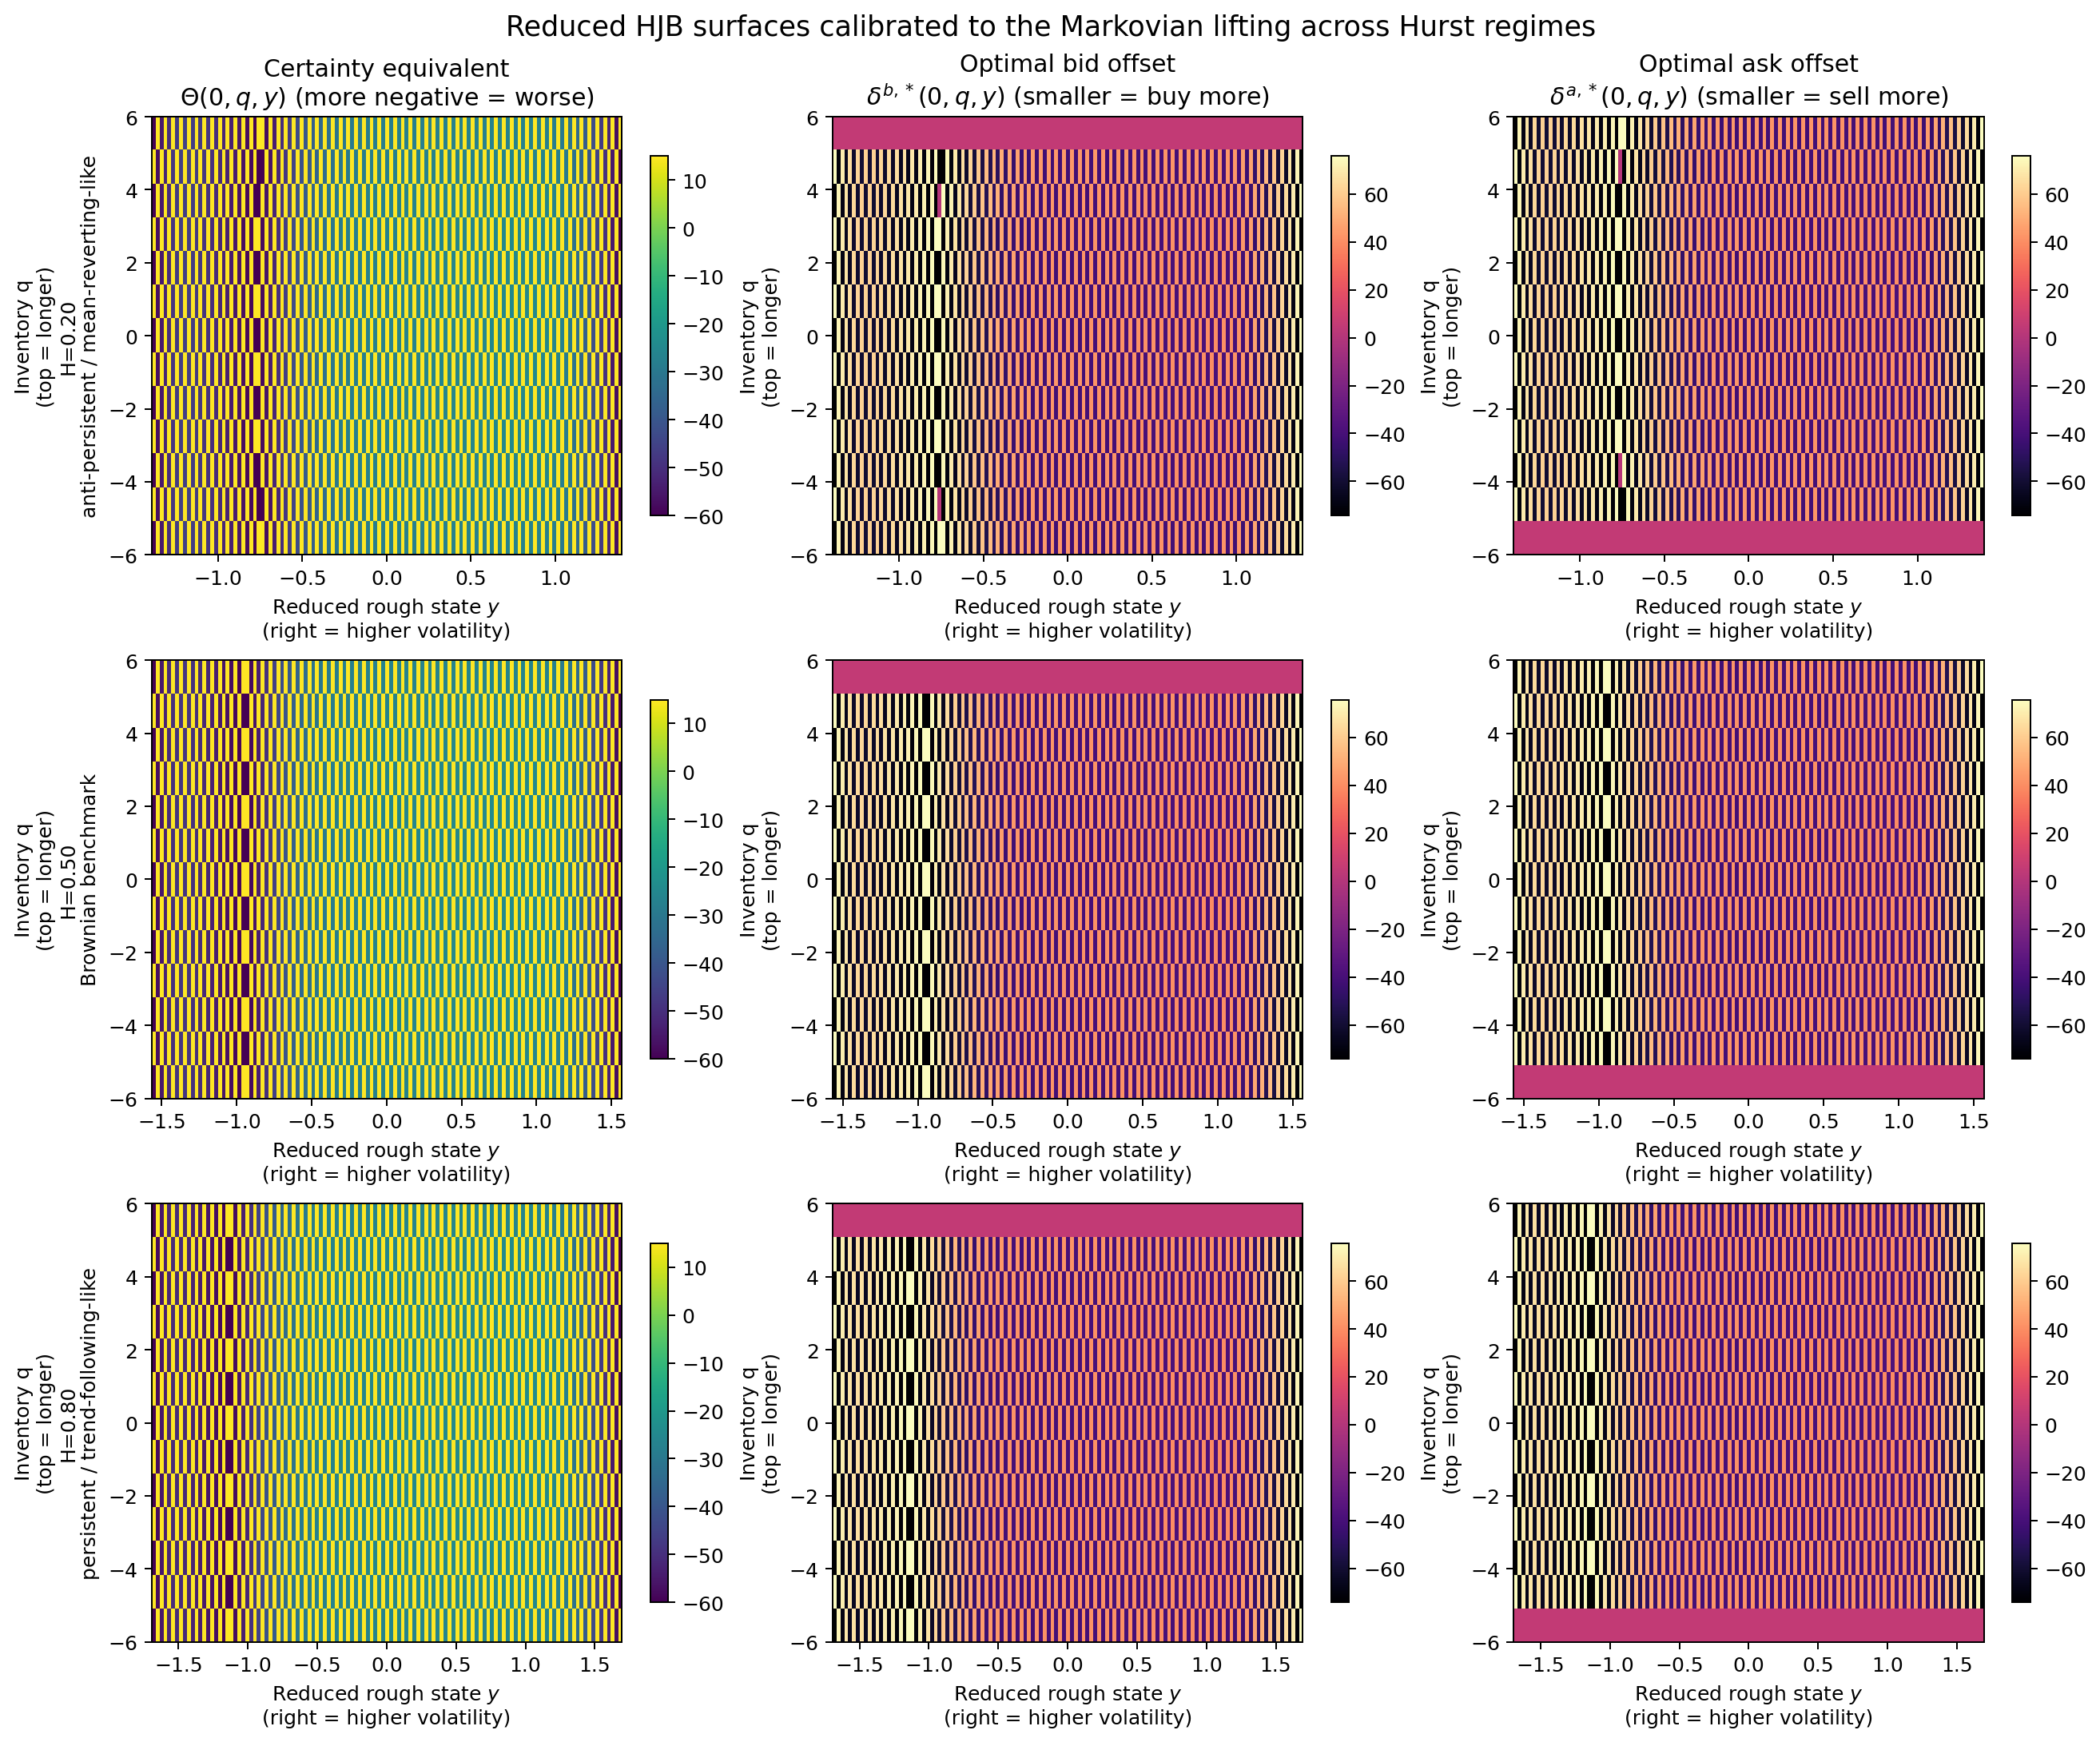
\includegraphics[width=\textwidth]{img/hft2-hjb_surfaces.png}
\caption{Reduced HJB surfaces across the three Hurst regimes. Each row corresponds to one lifted environment: \(H=0.2\) anti-persistent, \(H=0.5\) Brownian, and \(H=0.8\) persistent. The columns show the certainty-equivalent correction, the optimal bid offset, and the optimal ask offset at the initial time.}
\label{hft2-fig:hjb_surfaces}
\end{figure}

To read Figure~\ref{hft2-fig:hjb_surfaces}, fix one row first, so that \(H\) is held constant, and then move inside that row:
\begin{enumerate}[label=\arabic*.]
    \item The horizontal axis is the rough state \(y\). Moving to the right means a more stressed rough-volatility state and therefore a larger local variance forecast.
    \item The vertical axis is the inventory \(q\). Moving upward means the dealer is longer inventory; moving downward means the dealer is shorter inventory.
    \item In the first column, \(\Theta(0,q,y)\) is the continuation-value correction. More negative values mean that carrying that state forward is less attractive because future inventory risk and liquidation risk are more expensive.
    \item In the second column, \(\delta^{b,*}(0,q,y)\) is the optimal bid offset. A \emph{smaller} bid offset means the bid is closer to the mid-price, so the dealer buys more aggressively. A \emph{larger} bid offset means the dealer backs the bid away and becomes less willing to buy.
    \item In the third column, \(\delta^{a,*}(0,q,y)\) is the optimal ask offset. A \emph{smaller} ask offset means the ask is closer to the mid-price, so the dealer sells more aggressively. A \emph{larger} ask offset means the dealer is less willing to sell.
\end{enumerate}

The Avellaneda--Stoikov asymmetry is therefore read vertically. If one moves upward to positive inventory, the dealer should buy less aggressively and sell more aggressively: the bid offset widens, the ask offset tightens, and the certainty-equivalent surface deteriorates. If one moves downward to negative inventory, the pattern reverses. The effect of the rough state is read horizontally: moving toward larger \(y\) raises the volatility forecast, so both quotes tend to become more conservative overall, while the exact curvature changes across the three Hurst regimes.

The volatility diagnostics confirm that the environment remains genuinely stochastic in all three cases. The mean integrated variance changes only slightly, but the dispersion increases with \(H\), which is consistent with the fact that persistent regimes keep variance excursions alive for longer. This is why it is useful to report not only PnL and inventory, but also volatility statistics themselves.

\begin{table}[H]
\centering
\caption{Volatility diagnostics of the simulated environment across \(2{,}000\) trading days.}
\label{hft2-tab:hjb_vol_diagnostics}
\begin{tabular}{@{}lrrrr@{}}
\toprule
\(H\) & Mean realized vol & Std realized vol & Mean integrated var & Std integrated var \\
\midrule
0.20 & 1.096 & 0.081 & 1.209 & 0.155 \\
0.50 & 1.095 & 0.090 & 1.209 & 0.180 \\
0.80 & 1.095 & 0.098 & 1.208 & 0.199 \\
\bottomrule
\end{tabular}
\end{table}

Figure~\ref{hft2-fig:hjb_simulation} then collects one representative day for each regime. The left column shows the lifted rough state together with the induced local variance, the center column shows the inventory path from the open to the forced flat close, and the right column compares the end-of-day liquidated PnL distributions of the naive and HJB strategies. The reported pattern is shared by these three configurations: the HJB policy consistently keeps much less inventory into the close, which translates into a much smaller liquidation bill.

\begin{algorithm}[H]
\caption{Reading the close-out simulation figure}
\DontPrintSemicolon
\For{each simulated trading day}{
  update the lifted rough state and map it into local variance\;
  simulate the mid-price and order arrivals under common random numbers\;
  compare naive symmetric quoting with the HJB inventory-aware policy\;
  force terminal liquidation, record close-out cost, PnL, and inventory diagnostics\;
}
select one representative path per regime and plot it beside the Monte Carlo PnL histograms\;
\end{algorithm}

The representative path is now selected separately inside each regime, which is the natural choice once the forward simulation uses the full lifted state and the three Hurst cases no longer share the same effective trajectory. Table~\ref{hft2-tab:hjb_representative_path} makes the close-out mechanics explicit. In every regime the HJB policy still arrives at the close with materially smaller inventory and therefore a much smaller liquidation bill than the naive benchmark.

\begin{table}[H]
\centering
\caption{Representative regime-specific paths from Figure~\ref{hft2-fig:hjb_simulation}.}
\label{hft2-tab:hjb_representative_path}
\begin{tabular}{@{}lrrrrrrr@{}}
\toprule
\(H\) & Seed & \(q_{T^-}^{\mathrm{naive}}\) & \(q_{T^-}^{\mathrm{HJB}}\) & \(L^{\mathrm{naive}}\) & \(L^{\mathrm{HJB}}\) & PnL\(_{\mathrm{naive}}\) & PnL\(_{\mathrm{HJB}}\) \\
\midrule
0.20 & 218 & 4.000 & -1.000 & 6.290 & 1.032 & -1.349 & 2.533 \\
0.50 & 250 & 4.000 & 1.000 & 6.719 & 1.140 & 5.544 & 8.833 \\
0.80 & 235 & 6.000 & 2.000 & 11.816 & 2.499 & 1.087 & 2.886 \\
\bottomrule
\end{tabular}
\end{table}

\begin{figure}[H]
\centering
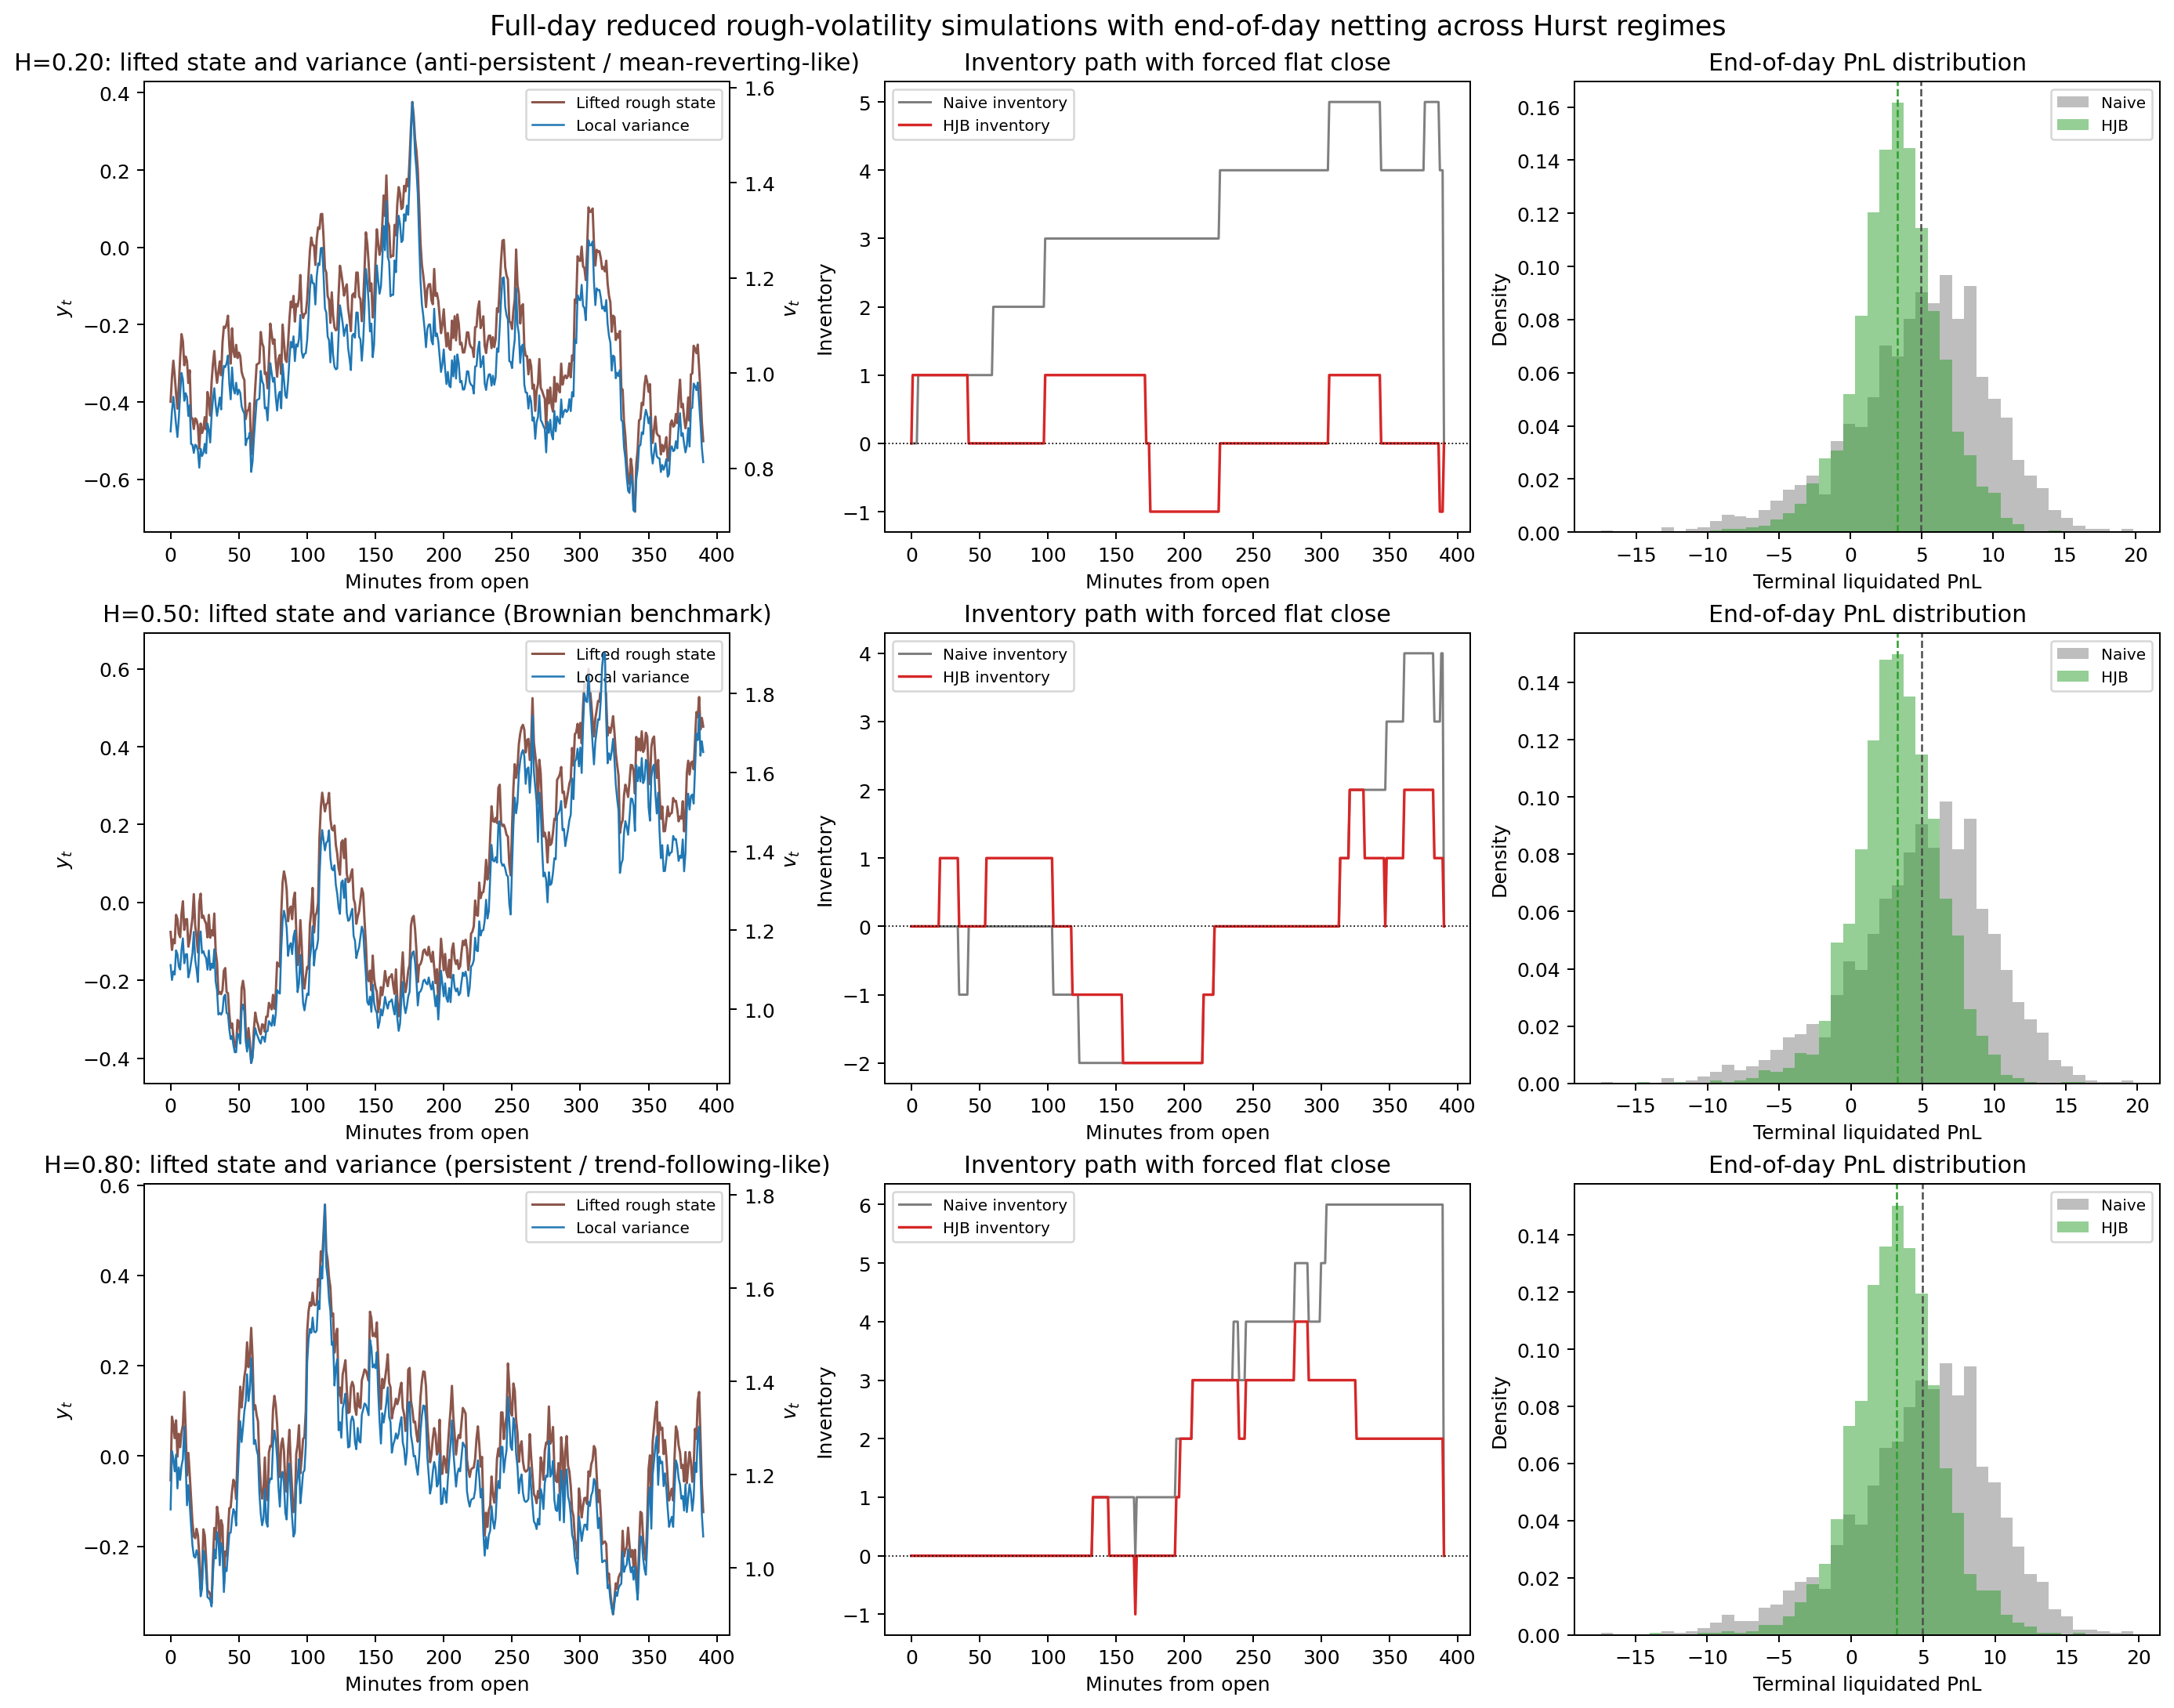
\includegraphics[width=\textwidth]{img/hft2-hjb_simulation.png}
\caption{Representative full-day simulations and Monte Carlo histograms across the three Hurst regimes. Rows correspond to \(H=0.2\), \(H=0.5\), and \(H=0.8\); columns show the lifted rough state and local variance, the inventory path with forced flat close, and the end-of-day liquidated PnL distribution.}
\label{hft2-fig:hjb_simulation}
\end{figure}

\subsection{Monte Carlo evidence and interpretation}

The full Monte Carlo comparison is reported in Tables~\ref{hft2-tab:hjb_mc_risk} and \ref{hft2-tab:hjb_mc_inventory}. Several points are worth separating carefully.

First, the naive benchmark keeps the larger \emph{mean} PnL in every regime. This is not a contradiction of Avellaneda--Stoikov. A symmetric spread-capture strategy can earn more average PnL precisely because it is willing to warehouse inventory and postpone the risk accounting until the close. The relevant question is therefore not ``which policy has the largest raw mean PnL?'', but rather ``what happens after one charges the close-out risk consistently?''

Second, on the dimensions that measure end-of-day inventory risk directly, the displayed historical HJB sample is better. In all three regimes the average pre-close inventory falls from about \(2.50\) to roughly \(0.55\), and the average liquidation cost falls from about \(3.99\) to roughly \(0.67\). The left tail also improves materially: the 5\% expected shortfall is less negative in every case.

\begin{table}[H]
\centering
\caption{Risk-adjusted Monte Carlo comparison with forced net-zero close (\(2{,}000\) sessions).}
\label{hft2-tab:hjb_mc_risk}
\begin{tabular}{@{}lrrrrrr@{}}
\toprule
\(H\) & Sharpe\(_N\) & Sharpe\(_H\) & CE\(_N\) & CE\(_H\) & ES\(_N\) & ES\(_H\) \\
\midrule
0.20 & 1.017 & 1.110 & 2.052 & 2.352 & -6.870 & -3.607 \\
0.50 & 1.017 & 1.082 & 2.056 & 2.208 & -6.865 & -3.734 \\
0.80 & 1.018 & 1.034 & 2.059 & 2.156 & -6.862 & -3.681 \\
\bottomrule
\end{tabular}
\end{table}

\begin{table}[H]
\centering
\caption{Inventory and liquidation metrics across the three Hurst regimes.}
\label{hft2-tab:hjb_mc_inventory}
\begin{tabular}{@{}lrrrrrr@{}}
\toprule
\(H\) & Mean PnL\(_N\) & Mean PnL\(_H\) & \(\E|q_{T^-}|_N\) & \(\E|q_{T^-}|_H\) & \(\E L_N\) & \(\E L_H\) \\
\midrule
0.20 & 4.955 & 3.309 & 2.504 & 0.547 & 3.990 & 0.654 \\
0.50 & 4.957 & 3.244 & 2.504 & 0.572 & 3.989 & 0.693 \\
0.80 & 4.958 & 3.173 & 2.504 & 0.549 & 3.988 & 0.667 \\
\bottomrule
\end{tabular}
\end{table}

The interpretation of the three regimes is now cleaner than before. For \(H=0.2\), the anti-persistent rough driver is the most favorable case for the HJB: the strategy gives up some mean PnL, but it improves Sharpe, certainty equivalent, and tail risk while dramatically shrinking the liquidation bill. For \(H=0.5\), the Brownian benchmark still leaves more raw spread-capture income to the naive policy, yet the historical sample favors the HJB on Sharpe, certainty equivalent, inventory discipline, and close-out cost. For \(H=0.8\), the persistent regime remains the hardest case in the sense that the risk-adjusted gain becomes smaller, but even there the reported HJB sample improves Sharpe, improves certainty equivalent, improves expected shortfall, and cuts liquidation cost by a large margin.

This is precisely where the earlier conceptual discussion matters. Avellaneda--Stoikov formulates a Markovian utility-maximization problem, not universal dominance in raw mean PnL after one changes the environment and adds forced end-of-day liquidation. In the present implementation, the naive benchmark still wins on average PnL because it warehouses inventory more aggressively. The historical HJB sample, however, has better reported metrics on the dimensions that actually price inventory risk correctly at the close.

The practical conclusion is therefore sharper. If one optimizes only raw mean PnL, the naive benchmark can still look attractive because it monetizes spread capture by tolerating much larger end-of-day inventory. Once one cares about close-out discipline, liquidation cost, certainty equivalent, and left-tail protection, the historical tables favor inventory-aware quotes on the reported risk-sensitive metrics in all three configurations.

These historical comparisons motivate the next check: whether the same inventory-control mechanism remains useful when the scalar solve uses positive bounded-control evolution instead of value clipping.
\section{A positive baseline in its scalar and lifted environments}
The historical clipped results above and the following positive-baseline replay answer different numerical questions. The policy and simulation configuration change, so a larger PnL here cannot be read as the isolated causal effect of repairing the solver. Within E1 and E2, however, the policy/naive comparison uses common shocks and consistent liquidation accounting.

The surfaces become a trading strategy through a feedback loop. At each simulated time, interpolate the solved certainty equivalent in $(t,Y)$ at the current discrete inventory, compute neighboring-inventory gains and apply the bounded Hamiltonian. The resulting offsets give $p_b=S-\delta_b$ and $p_a=S+\delta_a$. A dealer buy changes $(X,q)$ to $(X-p_b,q+1)$; a sale changes it to $(X+p_a,q-1)$. The next decision uses this updated inventory. A quote is not a guaranteed execution, and a price crossing is not the execution rule in this arrival-intensity model.

The illustrative simulator uses 3900 intervals over $T=1$, initial price 100, zero cash and inventory, and stationary volatility states. E1 uses the scalar OU model in which P2 was solved. E2 uses six common-noise OU factors with rates from 3 to 180 and normalized weights proportional to $\lambda^{-0.7}$. The price shock is independent of volatility. OU updates are exact on the grid; price and volatility are frozen during each interval's arrival processing, then price is advanced by its diffusion step. This splitting still requires time-step validation.

Candidate orders follow a Poisson process of rate $2A=28$, with equally likely sides and acceptance probability $\exp(-k\delta)$. Multiple candidates in an interval are processed sequentially, updating inventory and quotes after each fill. Both strategies share candidate counts, side marks, uniforms and the market path. The naive comparator uses constant symmetric offset $\log(1+\gamma/k)/\gamma$ and the same inventory limits. At $T$, liquidated wealth is $X_T+q_TS_T-L(q_T,Y_T)$ and inventory is reset to zero. This cost is charged once; no other fees are included.

Figure~\ref{hft3-fig:market-e2} provides the missing price--quote--inventory application. It uses seed 42 and path zero, fixed independently of which strategy wins. Green quotes determine the green inventory path through executions. The displayed path need not have smaller P2 inventory at every time; performance is assessed over the collection of paths. Crosses in the wealth panel show the terminal deduction rather than disguising it as continuous trading profit.

\begin{figure}[p]
\centering
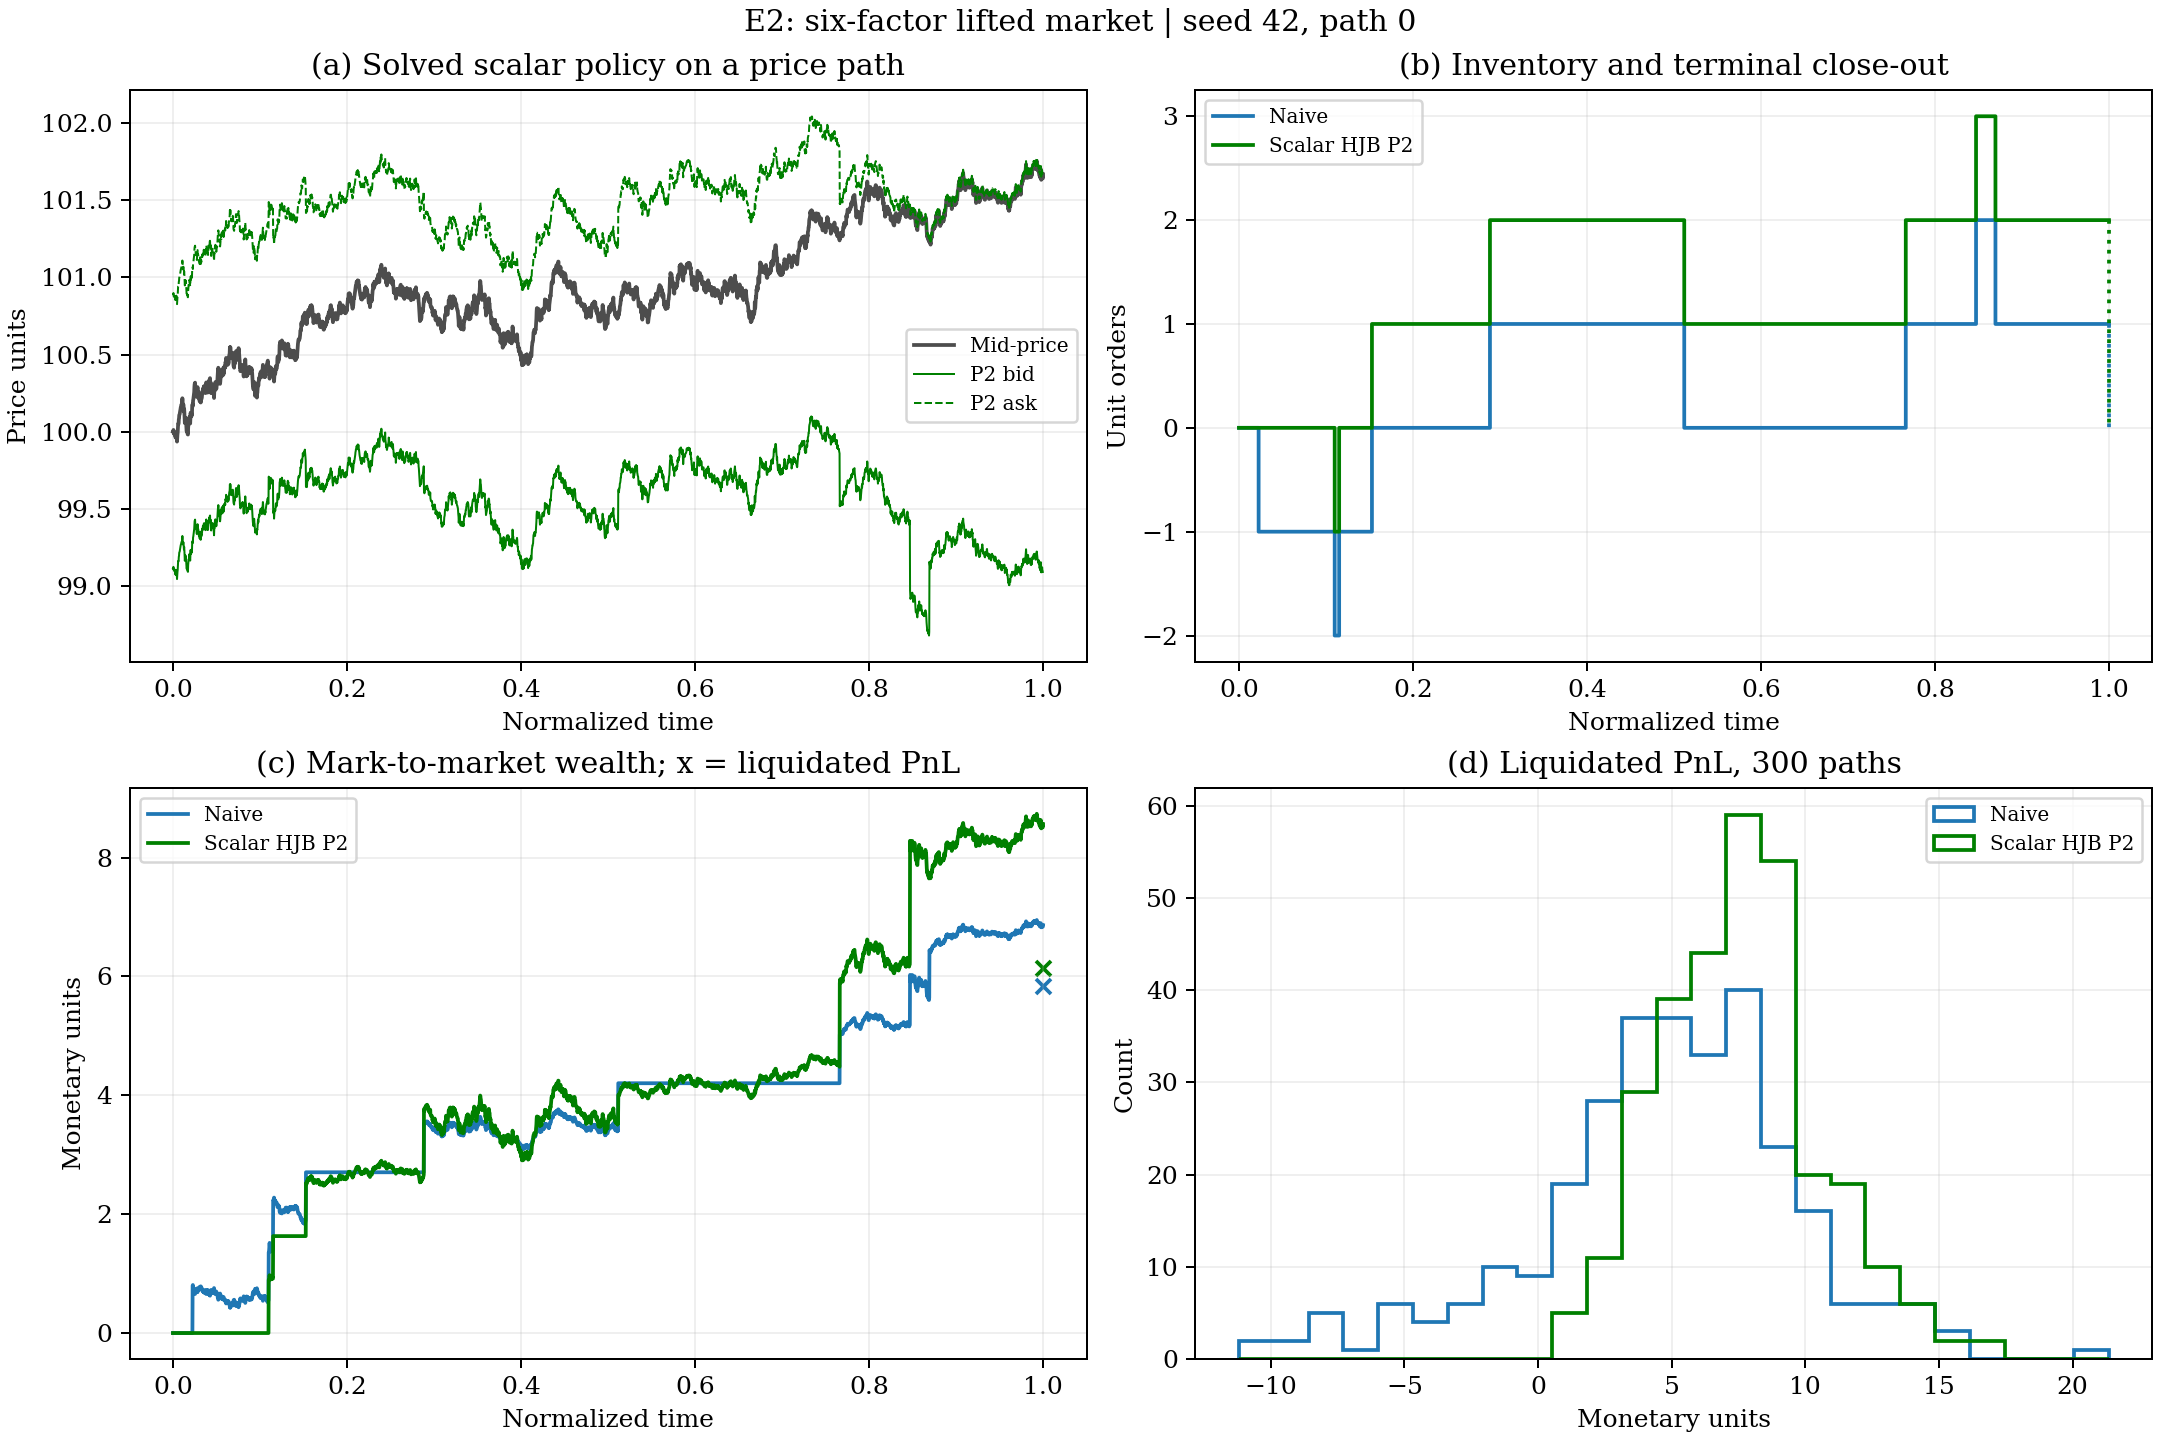
\includegraphics[width=\textwidth]{img/hft3-market_session_E2.png}
\caption{Baseline policy applied to the six-factor market E2. Top: price with P2 quotes and inventory for P2/naive. Bottom: marked wealth with liquidated terminal outcomes, and a common-bin histogram over 300 paired paths. Initial $S=100$, $X=q=0$, $T=1$, 3900 intervals, seed 42. This is P2 applied to a lifted environment, not a fitted HFT3 correction.}
\label{hft3-fig:market-e2}
\end{figure}

For E1, mean absolute inventory before liquidation is 2.433 for naive and 0.450 for P2; mean liquidated PnL is 5.445 and 7.724. For E2, these figures are 2.613 versus 0.427 and 4.792 versus 7.607. The mean paired PnL difference is 2.279 (standard error 0.215) in E1 and 2.816 (standard error 0.240) in E2. Comparisons are within each environment, not between the two sets of random paths. These synthetic baseline results do not demonstrate a correction benefit, global optimality or computational efficiency.

Checks enforce inventory limits, side disabling, exact-grid interpolation and the cash/inventory accounting identity, with maximum floating-point discrepancy $1.28\times10^{-13}$. No lookup leaves the exported state domain in these runs. The nearly singular OU innovation covariance is factored spectrally, removing only roundoff-negative eigenvalues: reconstruction error is $4.34\times10^{-19}$. The independent HJB residual, interpolation refinement and simulation-step convergence remain open. Consequently this experiment is an illustrative application, not the final validation gate for fitting P3.

\clearpage

\section{Adding stochastic covariance to separate policies}
The previous experiment tested the scalar policy against symmetric quotes. We now hold the positive baseline fixed and compare separate asset policies with the explicit covariance proxy from Chapter~\ref{ch:control}. This isolates a cross-inventory modification, not a transition from a Markovian to a non-Markovian model: the full twelve-factor environment remains finite-dimensional and Markovian.

Both strategies begin with $q=(3,0)$, prices $(100,100)$ and cash $-300$, so initial marked wealth is zero. This deliberately exposes the cross-asset response to a long A position. For each asset the inventory limit is six units and the arrival parameters remain $A=14$, $k=1.15$. One marked Poisson candidate stream of total rate 56 chooses asset and side uniformly; acceptance probability is $e^{-k\delta}$. Inventory and both assets' quotes are updated after every accepted candidate. Common candidates and exogenous shocks pair the two policies. Price and volatility remain frozen during each interval's arrivals, followed by diffusion updates. All assets are liquidated at $T$ and the sum of the two declared liquidation costs is charged once.

Figure~\ref{hft3-fig:multi-inventory} shows path zero under seed 73, fixed independently of the outcomes. Purple B inventory initially becomes short while A is long. Later, when positions and prices have evolved differently, the same policy can carry more risk than the separate policy. The selected path is illustrative; it is not required to exhibit the average ranking at every time.

\begin{figure}[p]
\centering
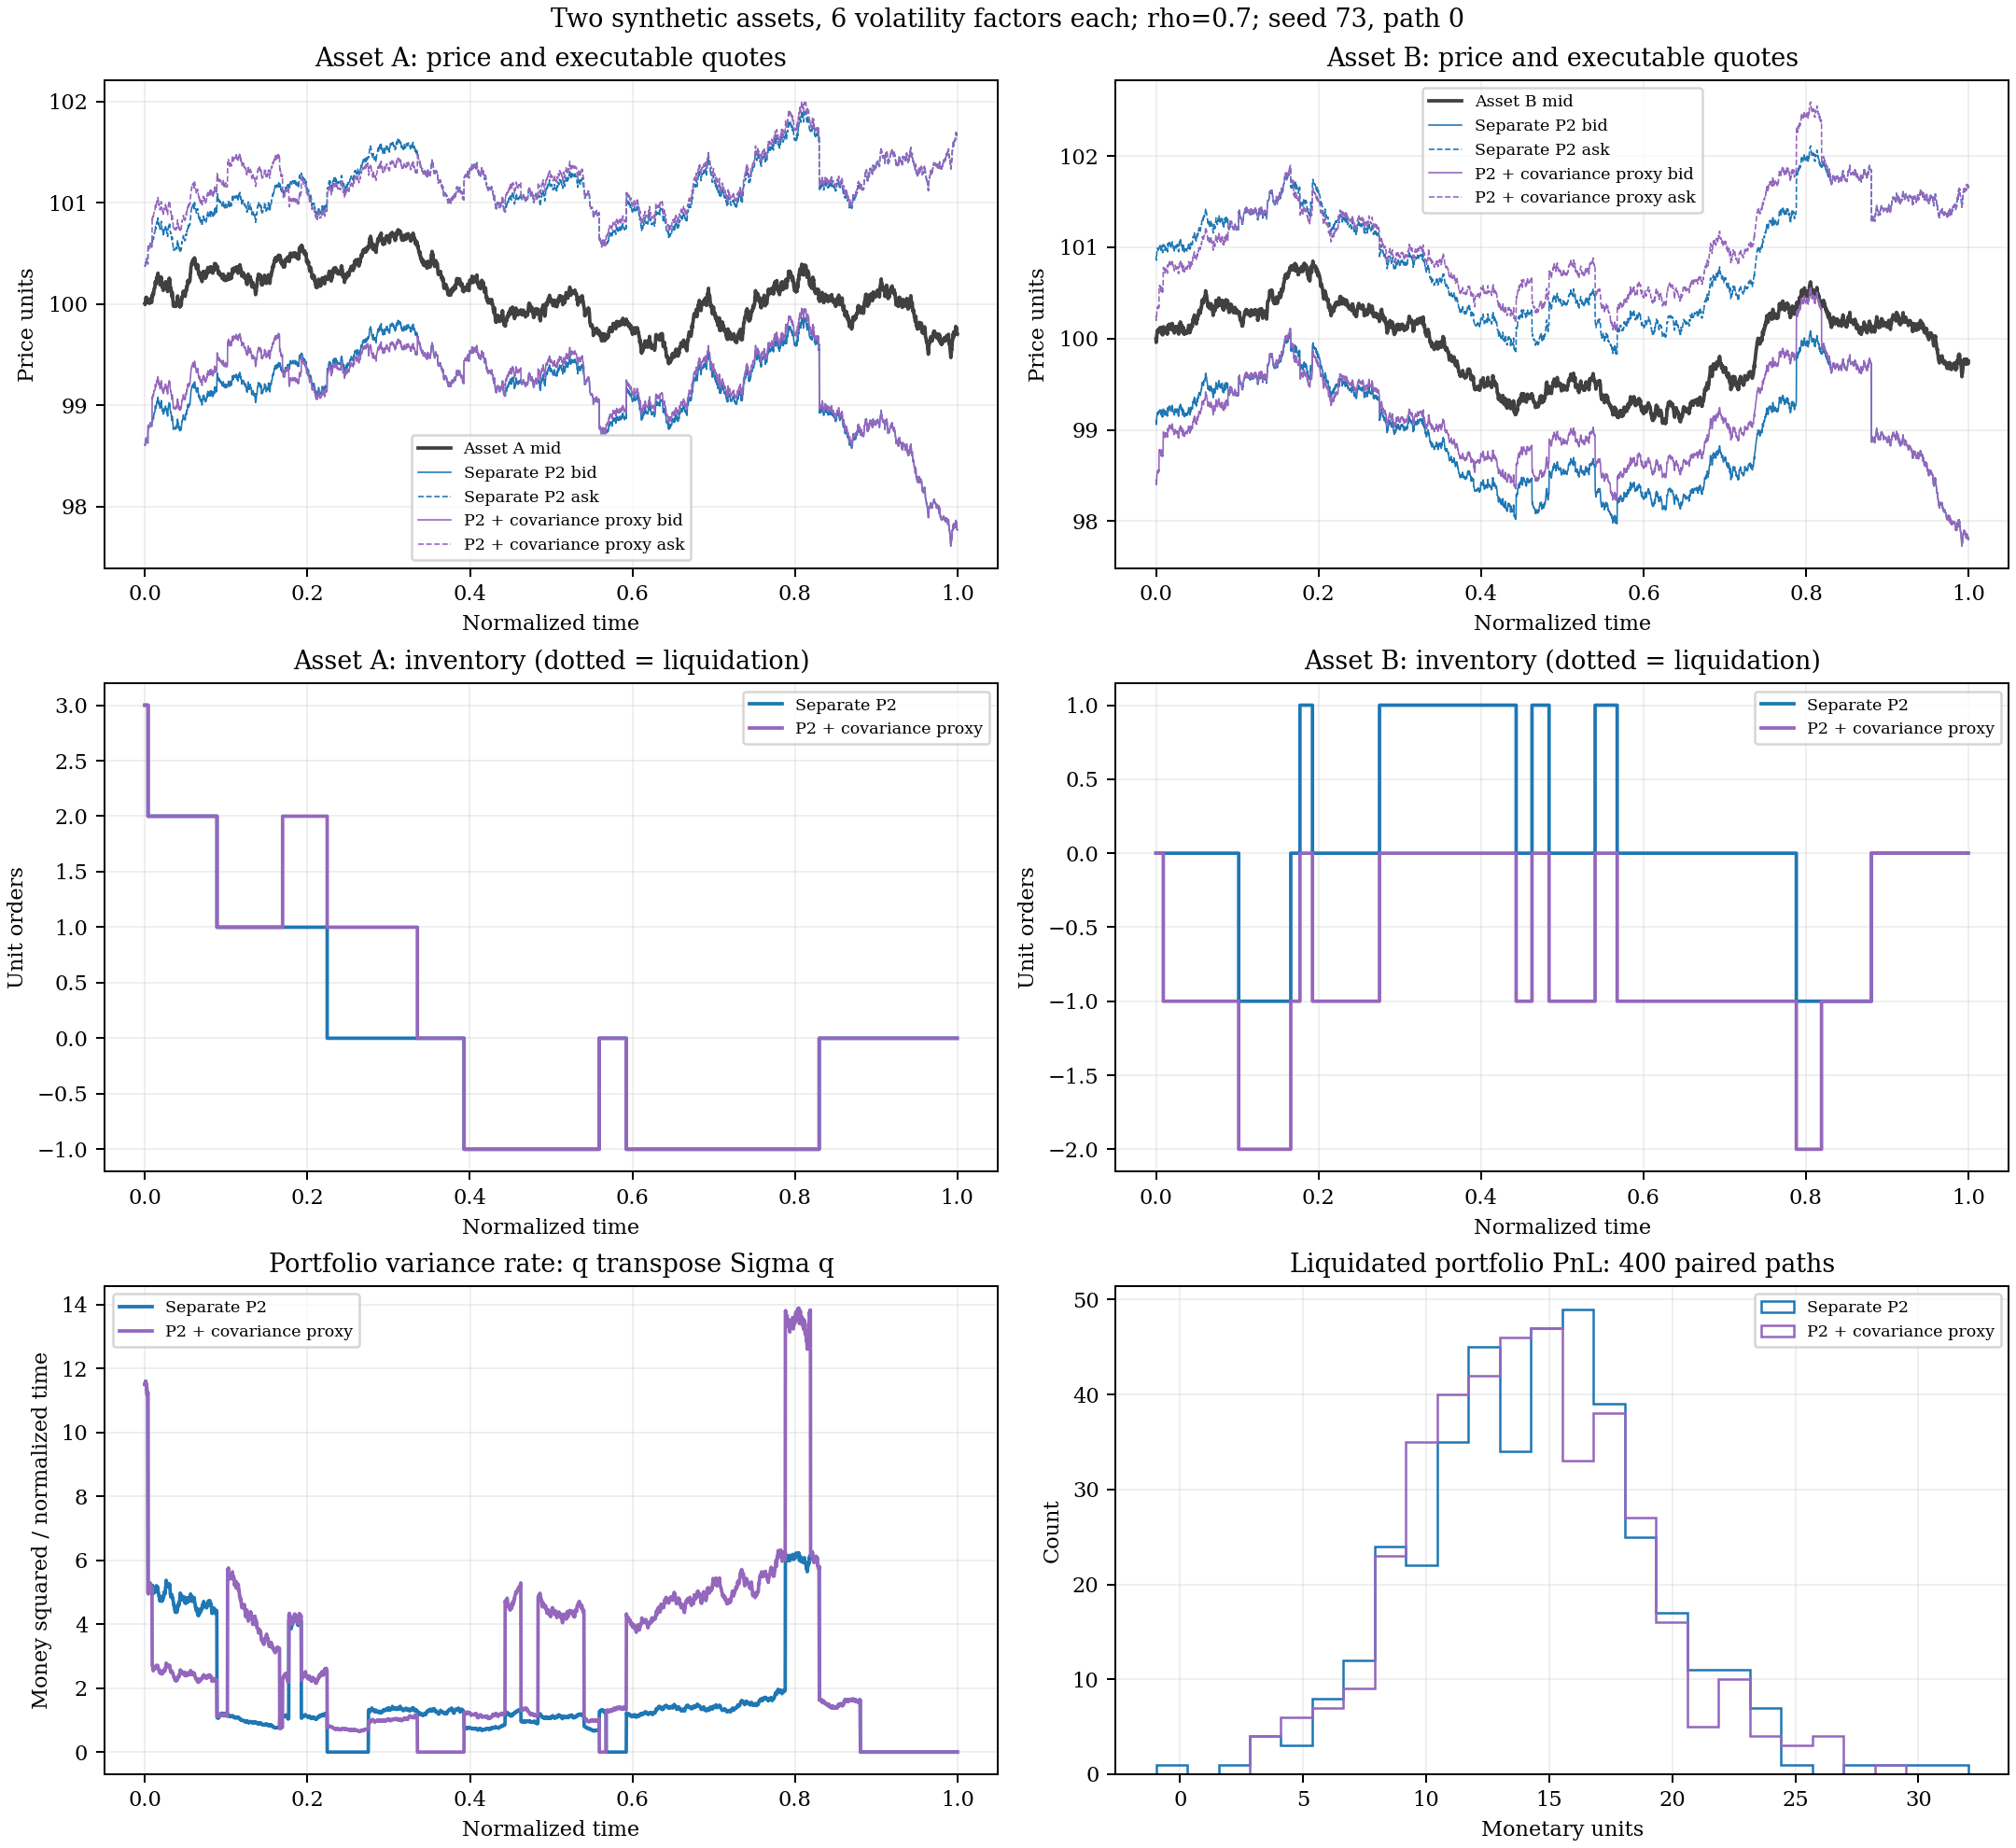
\includegraphics[width=\textwidth]{img/hft3-multiasset_inventory.png}
\caption{Two-asset application of separate P2 and P2 plus the covariance proxy. Top: both price paths and executable quotes. Middle: both inventories, with terminal liquidation dotted. Bottom: portfolio variance rate on the fixed illustrative path and liquidated PnL over 400 paired paths. Main run: 3900 intervals, price correlation 0.7, volatility-driver correlation 0.35, seed 73. The proxy is not the fitted residual-corrected policy P3.}
\label{hft3-fig:multi-inventory}
\end{figure}

For the main 400-path experiment, the results are
\begin{center}
\begin{tabular}{@{}lrr@{}}
\toprule
Metric & Separate P2 & Covariance proxy\\
\midrule
Mean $\int_0^Tq_t^\top\Sigma_tq_t\,dt$ & 5.8443 & 4.9608\\
Mean liquidated PnL & 14.4335 & 14.0905\\
Sample CARA certainty equivalent & 12.3054 & 12.2345\\
Mean $|q_A|$ before liquidation & 0.5275 & 0.5300\\
Mean $|q_B|$ before liquidation & 0.4825 & 0.5200\\
\bottomrule
\end{tabular}
\end{center}
The integrated-risk difference (proxy minus separate) is $-0.8835$, with paired standard error 0.1085: approximately 15.1\% lower mean integrated variance. This metric measures accumulated instantaneous inventory risk, not the sample variance of terminal PnL. The mean PnL difference is $-0.3430$, with paired standard error 0.0908. The sample certainty equivalent $-\log(\operatorname{mean}e^{-\gamma\mathrm{PnL}})/\gamma$ also decreases slightly; the conditional bootstrap interval for this nonlinear statistic is reported in the comparative-results chapter. The experiment therefore does not establish an improvement in the CARA objective. It shows a risk--revenue trade-off and motivates a better correction rather than validating this proxy as optimal.

A 1950-interval diagnostic with 400 paths has the same qualitative average trade-off: integrated variance 5.9781 versus 5.2543, PnL 13.9323 versus 13.6632. These two resolutions do not certify convergence. Reusing a seed at a different step count does not couple identical Brownian paths across resolutions; pairing is within each run. A separate zero-price-correlation regression produces identical inventories, cash and outcomes for both policies, even though the volatility drivers retain correlation 0.35. Thus this correction isolates price-covariance inventory coupling, not every source of dependence.
\section{A stochastic-covariance residual diagnostic}
For $\theta_{sep}=\theta_0(t,q_A,Y_A)+\theta_0(t,q_B,Y_B)$ and $C=-\gamma(T-t)\Sigma_{AB}q_Aq_B$, the complete operator is evaluated with $\partial_t C$, $\nabla C$, $D^2 C$, mixed factor covariances and changed nonlinear arrival gains. Since $\Sigma_{AB}\propto\exp(\beta(Y_A+Y_B)/2)$, $\partial_{Z_{im}}C=(\beta w_m/2)C$ and $D^2 C=Caa^\top$, with $a_{im}=\beta w_m/2$. The covariance terms cannot be discarded as if the covariance were fixed over the control horizon.
On 1379 held-out interior states from 1500 samples (seed 20261013), the sum of reduced-operator residuals has RMS 0.004638; the full separate-policy residual has RMS 2.481440; the full covariance-proxy residual has RMS 5.069320. The proxy therefore worsens this diagnostic. A current-covariance hedge is not a full residual correction.
The baseline derivatives are reconstructed by cubic time/state splines from the existing export. This diagnostic is not an independently converged reference solution, a bound on value error, or a certification of derivative convergence. It does not justify fitting P3 before the remaining numerical gates.
\section{Separated refinement and sampling uncertainty}
Nine positive-baseline solves separate temporal refinement (4680/9360/18720 effective steps at 241 nodes and 5SD), fixed-spacing domain refinement (4/5/6SD with 193/241/289 nodes) and spatial refinement (81/161/241 nodes at 5SD). Non-reference configurations are compared below with the finest configuration in their family, at $t=0,0.5$, over every inventory and common interior interpolation points. These are finite-resolution differences, not rigorous errors.
\begin{table}[ht]\centering\small
\begin{tabular}{lrrr}\toprule Study & Configuration & Max value diff. & Max offset diff.\\\midrule
temporal & 4680 & 0.0028724 & 0.0008224 \\
temporal & 9360 & 0.0009573 & 0.0002740 \\
fixed spacing domain & 4 & 0.0001309 & 0.0000465 \\
fixed spacing domain & 5 & 0.0000014 & 0.0000003 \\
spatial & 81 & 0.0012923 & 0.0010935 \\
spatial & 161 & 0.0003235 & 0.0002459 \\
\bottomrule\end{tabular}
\caption{Refinement in separate directions. Configuration is step count, domain SD, or node count according to the study.}
\end{table}
For the two-asset experiment, 10,000 paired bootstrap resamples give a covariance-minus-separate certainty-equivalent difference -0.070843, with percentile 95\% interval $[-0.398632,0.288272]$. The interval contains zero: the negative sample difference does not establish a population utility loss. This is conditional sampling uncertainty, not model/parameter uncertainty.
The preceding classical generator freeze used 1000 multivariate paths and a different correlation matrix. A separate replay now uses the supplied 3000-path configuration, with correlations $\rho_{AB}=0.65$, $\rho_{AC}=-0.55$ and $\rho_{BC}=-0.35$. It reproduces mean terminal PnL 158.709/154.556, PnL standard deviation 16.439/10.547, gross terminal inventory 21.949/11.203 and terminal risk norm 17.051/7.419 to the article's displayed rounding. The scalar 5000-path ABM/GBM figures also reproduce their reported summary statistics. Earlier configurations remain separately preserved.

\section{What the experiments jointly establish}
Across the diffusion and historical finite-lift studies, inventory-sensitive quotes give up some sample mean revenue while lowering exposure or liquidation costs. The positive-baseline E1/E2 replay instead reports higher mean liquidated PnL than its own naive comparator. The covariance proxy reduces accumulated price risk but lowers sample PnL/CE and increases the reconstructed full residual. These are compatible outcomes because the comparator, state representation and objective differ.

The shared lesson is methodological: use the same accounting inside a comparison and assess utility and the declared operator in addition to inventory risk. A lower terminal-inventory statistic does not imply a better CARA objective; a small reduced residual does not imply a small full residual; and a finite-grid comparison does not supply a convergence certificate. This is the evidence on which the correction design in the next chapter must build.
